%%%%%%%%%%%%%% Figure 1: 8-K Merging Process
\begin{figure}
	\caption{8-K Merging Process} \label{fig1}
	\begin{center}
		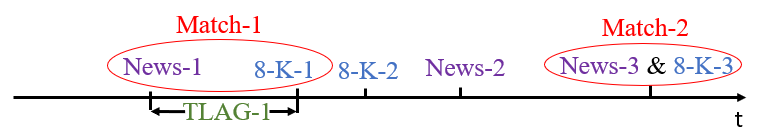
\includegraphics[scale=0.6]{../output/fig/fig1_matching.png}
	\end{center}
\end{figure}

Figuer 1 illustrates the 8-K sample matching process. We match every news day to its first posterior 8-K day, ignoring the successive 8-K days (if any) between two news days (Match-1), or in some cases the 8-K day coincides with news day (Match-2).

%%%%%%%%%%%%%% Figure 2: Sample Selection Process
% Table generated by Excel2LaTeX from sheet 'Fig2'
\begin{table}[htbp] \label{fig2}
  \centering
    \begin{tabular}{lr}
    \multicolumn{2}{c}{Figure 2: Sample Selection Process} \\
    \multicolumn{2}{c}{10-Q} \\
    Numer of observations: &  \\
    Retrieved from EDGAR & 575,579 \\
    After merging with COMP and CRSP data & 190,341 \\
    After merging with I\textbackslash{}B\textbackslash{}E\textbackslash{}S and segment data & 110,114 \\
    After dropping obs. with missing values in key variables and screening & \textbf{91,606} \\
      &  \\
    \multicolumn{2}{c}{8-K} \\
    Numer of observations: &  \\
    Retrieved from EDGAR & 1,489,626 \\
    After merging and matching with COMP and CRSP data & 390,698 \\
    After dropping obs. with missing values in key variables and screening & \textbf{244,401} \\
    After filtering obs. with TLAG smaller or equal to 4 (8-K restricted sample) & \textbf{61,443} \\
    \end{tabular}%
\end{table}%
 \label{fig2}

%%%%%%%%%%%%%% Figure 3: 8-K Item Distribution
\setcounter{figure}{2}
\begin{figure}[htbp]
	\begin{center}
		\caption{8-K Item Distribution} \label{fig3}
		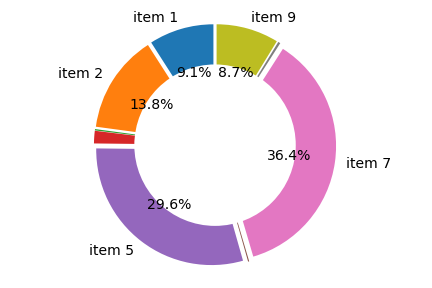
\includegraphics[scale=0.5]{../output/fig/fig3_8-K_before.png}
		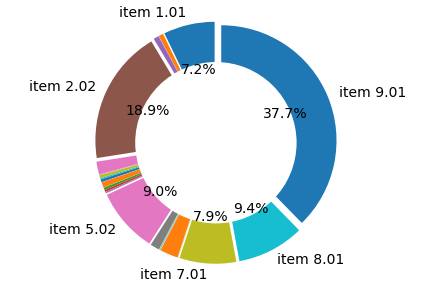
\includegraphics[scale=0.5]{../output/fig/fig3_8-K_after.png}
	\end{center}
\end{figure}

Figuer 3 illustrates the 8-K item distribution before (left) and after (right) May 23rd of 2004, respectively. Each share of pie chart shows the percentage of corporate events reported under each 8-K items. See 8-K item list in \hyperref[appd]{Appendix D}.